\documentclass[bigger]{beamer}

\usepackage{booktabs}
\useinnertheme{rounded}
\usecolortheme{crane}
\setbeamerfont{block title}{size={}}
\usepackage[autolanguage]{numprint}

\usetheme{Proso}

\title{Impact of Question Difficulty on Engagement and Learning}

\author{Jan Papou\v{s}ek, \textbf{V\'it Stanislav}, Radek Pel\'anek \\
%Masaryk University Brno\\
%Czech Republic
}

\date{ITS 2016}
 
\begin{document}

\frame{\titlepage}


\begin{frame}
	\begin{center}
    {\Huge Example scenario} 
	\end{center}
\end{frame}

\begin{frame}
  \frametitle{Example scenario}
	\noindent\makebox[\textwidth]{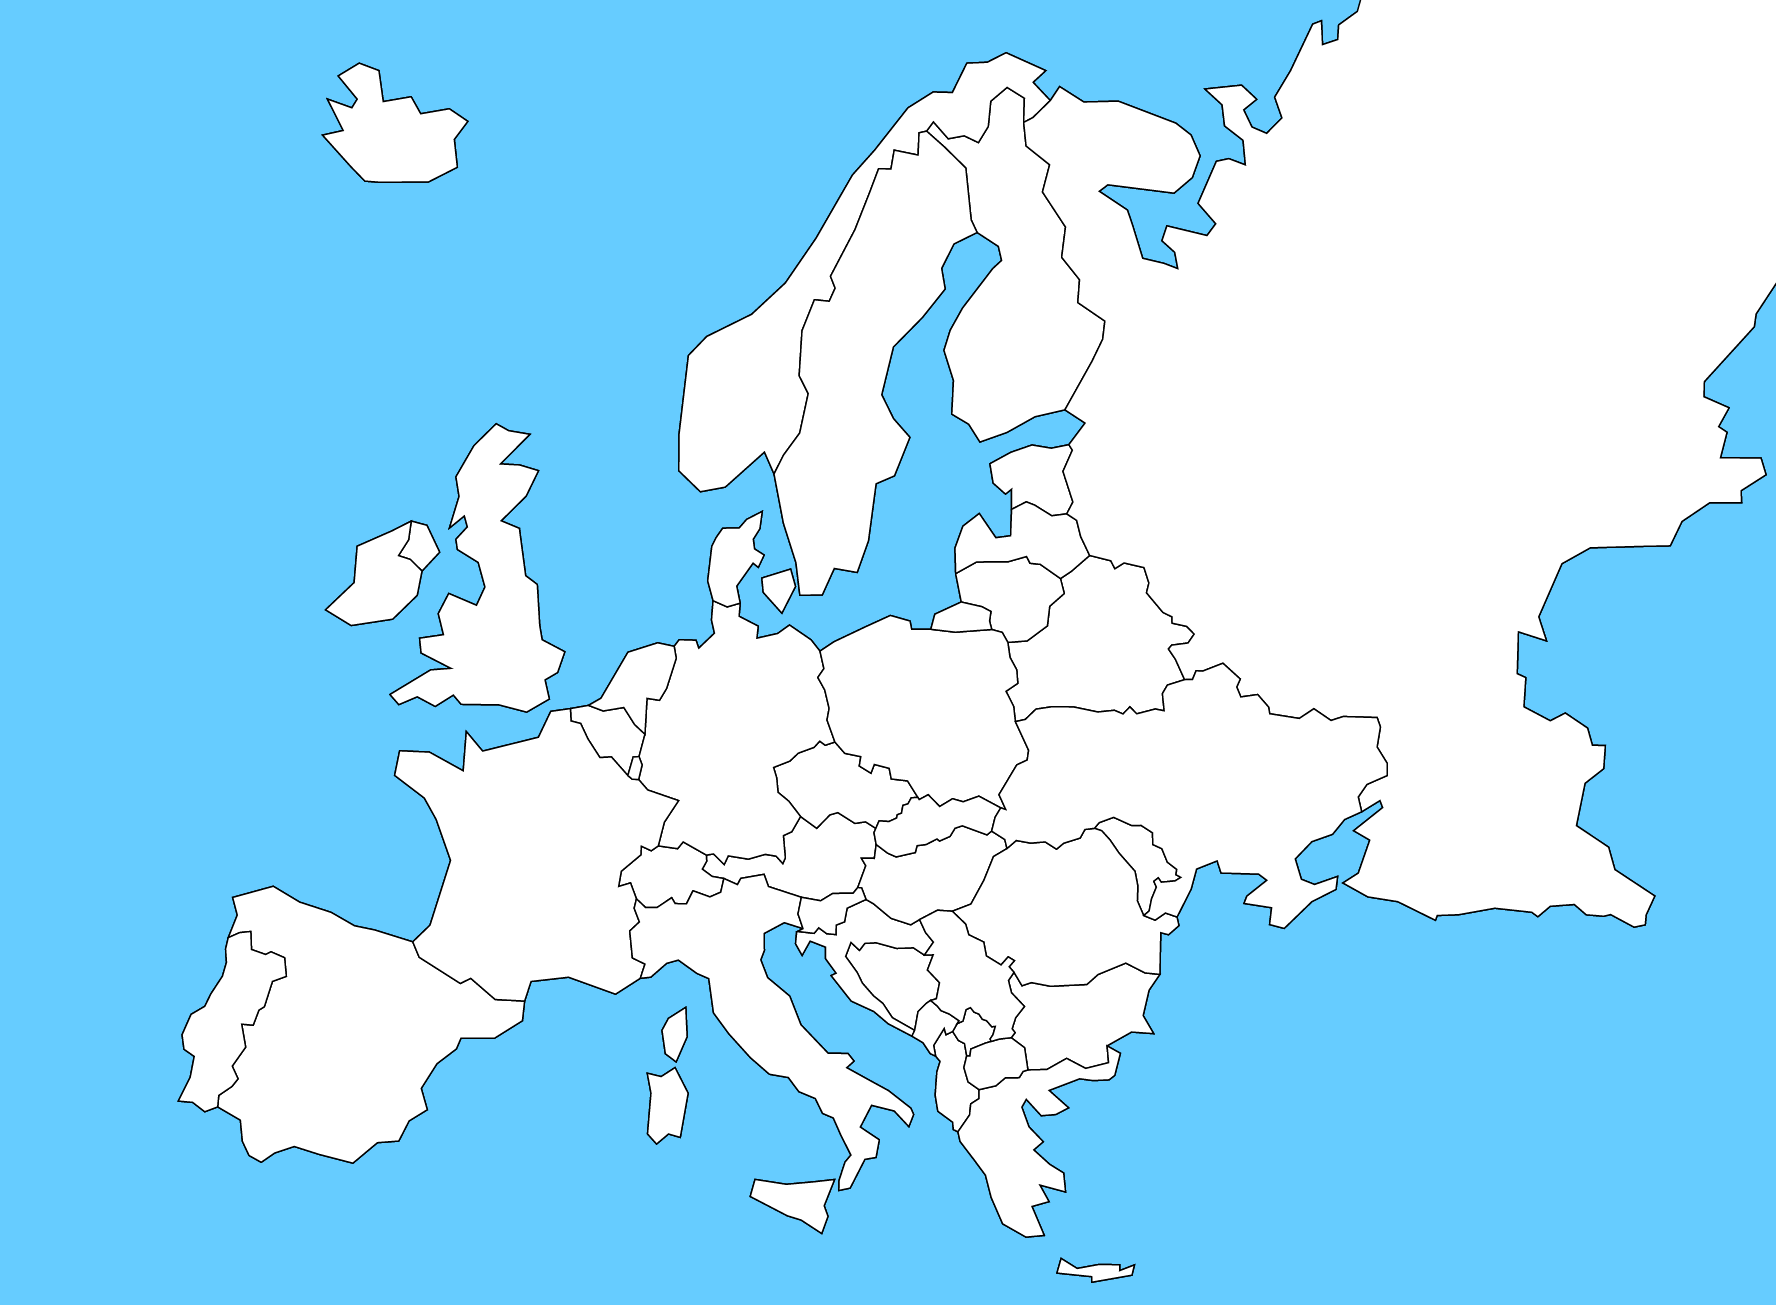
\includegraphics[width=\paperwidth]{img/europe-state}}
\end{frame}

\begin{frame}
  \frametitle{Example scenario}
	\noindent\makebox[\textwidth]{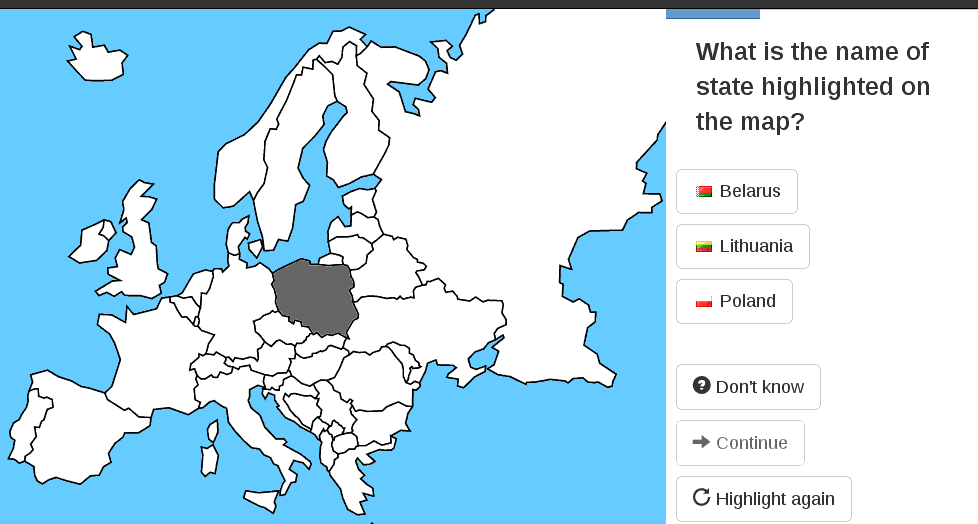
\includegraphics[width=\paperwidth]{img/practice-example-en}}
\end{frame}

\begin{frame}
  \frametitle{Example scenario}
    \begin{center}
      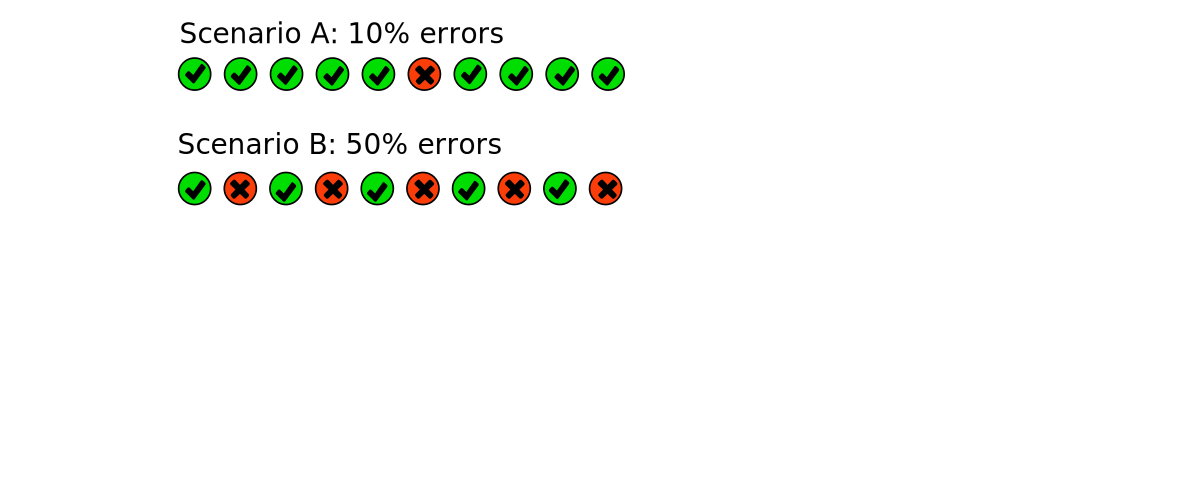
\includegraphics[width=0.8\textwidth]{img/error_rate_scenarios}
    \end{center}
\end{frame}

\begin{frame}
  \frametitle{Research question}
	\begin{center}
    {\Huge What is optimal question difficulty?} 

		\bigskip
    {\Huge ...for engagement vs. for learning}
	\end{center}
\end{frame}

\begin{frame}
	\frametitle{Prior research}
	\begin{itemize}
	  \item Abuhamdeh et al. (2012): Inverted U hypothesis
	  \item Lomas et al. (2013): easier problems lead to higher engagement, but lower learning.
	  \item Jansen et al. (2013): easiest condition leads to the best learning
	\end{itemize}
\end{frame}

\begin{frame}
	\begin{center}
    {\Huge Experimental setting} 
	\end{center}
\end{frame}

\begin{frame}
  \frametitle{outlinemaps.org}
	\noindent\makebox[\textwidth]{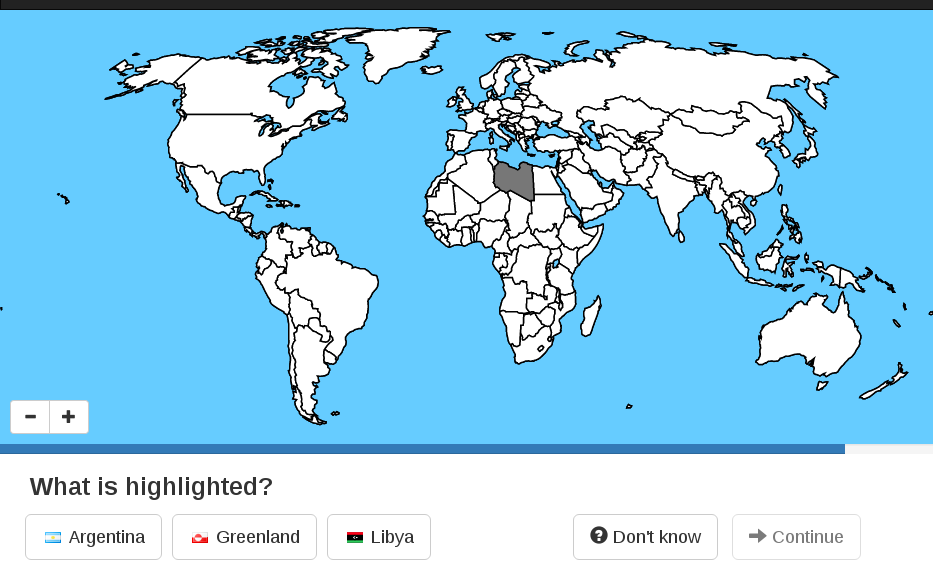
\includegraphics[width=\paperwidth]{img/slepemapy_world_practice}}
\end{frame}

\begin{frame}
  \frametitle{outlinemaps.org}
	\noindent\makebox[\textwidth]{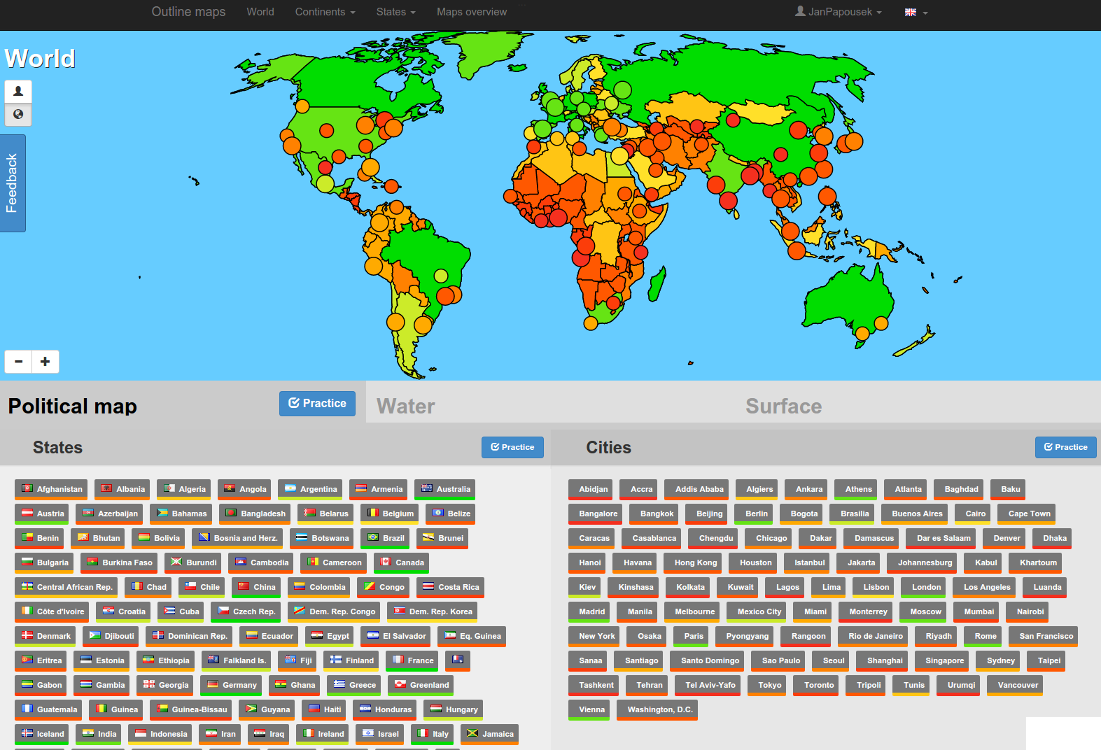
\includegraphics[width=\paperwidth]{img/slepemapy_world}}
\end{frame}

\begin{frame}
	\frametitle{How do we aim?}
	\begin{itemize}
		\item Prediction from a model
    \begin{itemize}
      \item Russia vs. Serbia
    \end{itemize}
		\item Number of options
    \begin{itemize}
      \item Open question vs. 2-options MCQ
    \end{itemize}
	\end{itemize}
\end{frame}

\begin{frame}
  \frametitle{Experimental setting}
	\begin{itemize}
		\item online AB experiment
		\item new users were randomly assigned to one of the studied conditions
	\end{itemize}
	\begin{center}
		\begin{tabular}{ccc}
			\textbf{Target error rate} & \textbf{notation} \\
			\toprule
			 5\% & C05 \\
			 20\%   & C20 \\
			 35\% & C35 \\
			 50\%   & C50 \\
			\bottomrule
		\end{tabular}
	\end{center}
\end{frame}

\begin{frame}
	\begin{center}
    {\Huge Collected data} 
	\end{center}
\end{frame}

\begin{frame}
	\frametitle{Collected data}
	\begin{itemize}
		\item November 2015 to January 2016
		\item \numprint{3300000} answers from \numprint{37000} learners
		\item majority of users:
			\begin{itemize}
				\item Czech Republic (84 \%)
				\item Slovakia (8 \%)
			\end{itemize}
	\end{itemize}
\end{frame}

\begin{frame}
  \frametitle{Contexts}
  \only<1>{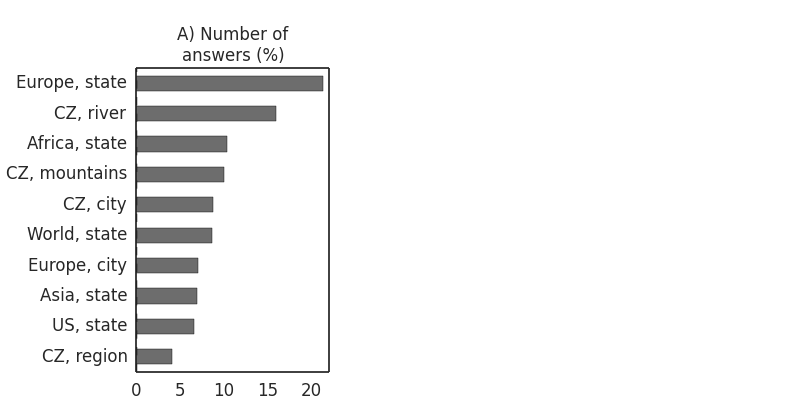
\includegraphics[width=\textwidth]{img/stats_by_context_ab_1}}
  \only<2>{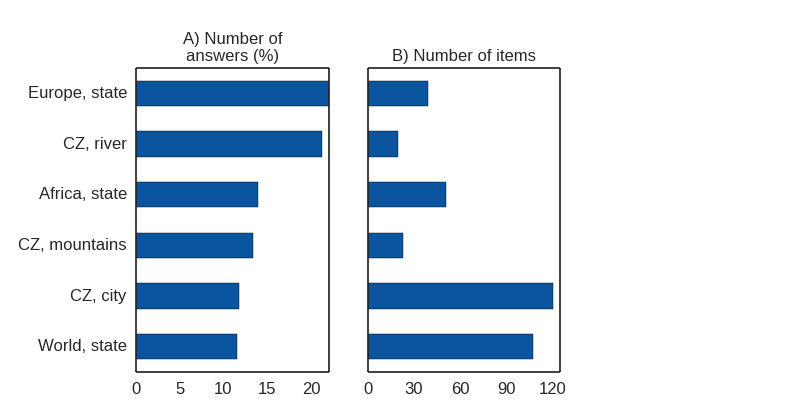
\includegraphics[width=\textwidth]{img/stats_by_context_ab_2}}
  \only<3>{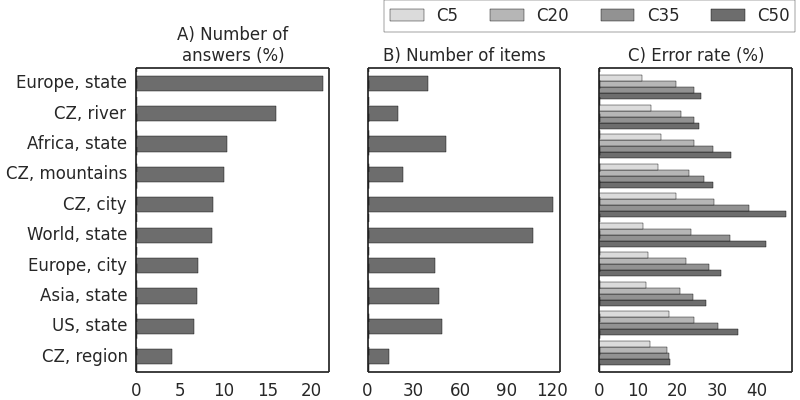
\includegraphics[width=\textwidth]{img/stats_by_context_ab}}
\end{frame}

\begin{frame}
	\begin{center}
    {\Huge Impact on Engagement} 
	\end{center}
\end{frame}


\begin{frame}
  \frametitle{Survival curve}
  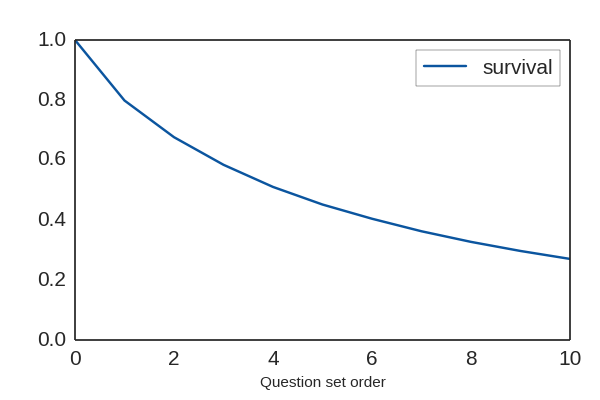
\includegraphics[width=\textwidth]{img/survival_curve_grouped}
\end{frame}

\begin{frame}
  \frametitle{Survival curve}
  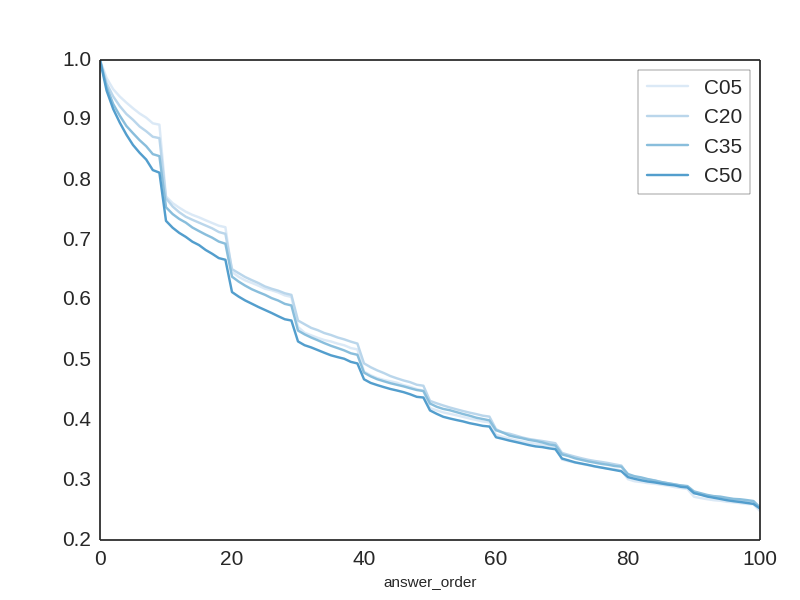
\includegraphics[width=\textwidth]{img/survival_curve_by_ab}
\end{frame}


\begin{frame}
  \frametitle{Survival}
  \only<1>{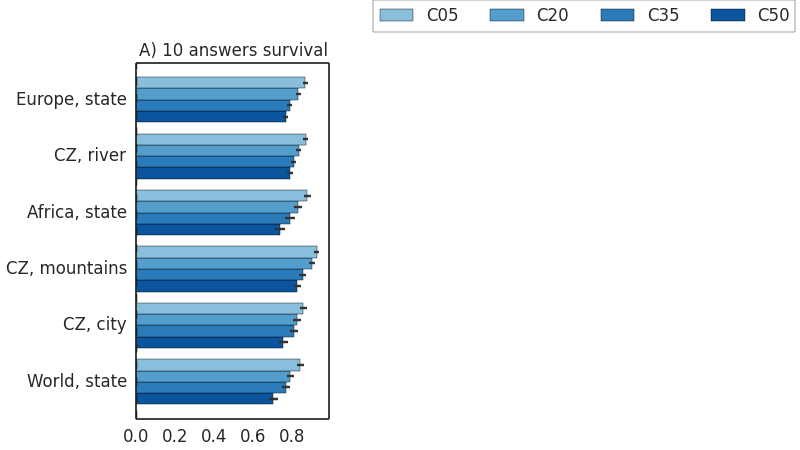
\includegraphics[width=\textwidth]{img/survival_by_context_ab_1}}
  \only<2>{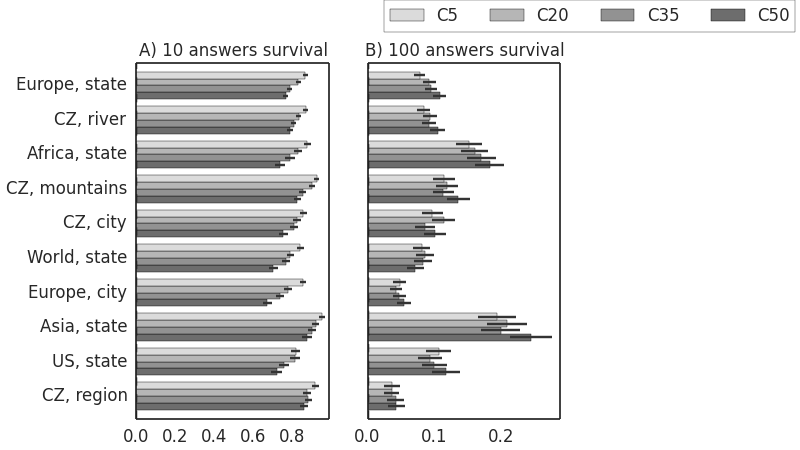
\includegraphics[width=\textwidth]{img/survival_by_context_ab_2}}
  \only<3>{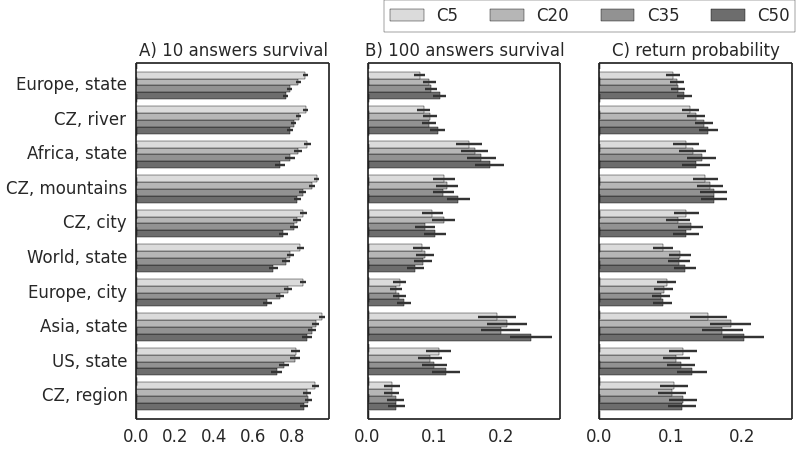
\includegraphics[width=\textwidth]{img/survival_by_context_ab}}
\end{frame}


\begin{frame}
  \frametitle{User rating}
  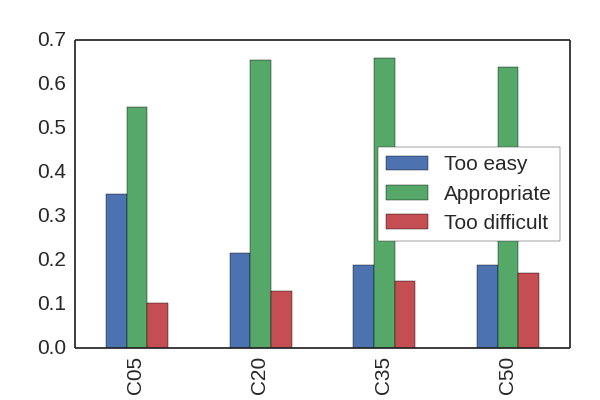
\includegraphics[width=\textwidth]{img/rating_by_ab}
\end{frame}

\begin{frame}
	\begin{center}
    {\Huge Impact on Learning} 
	\end{center}
\end{frame}


\begin{frame}
  \frametitle{Reference questions}
  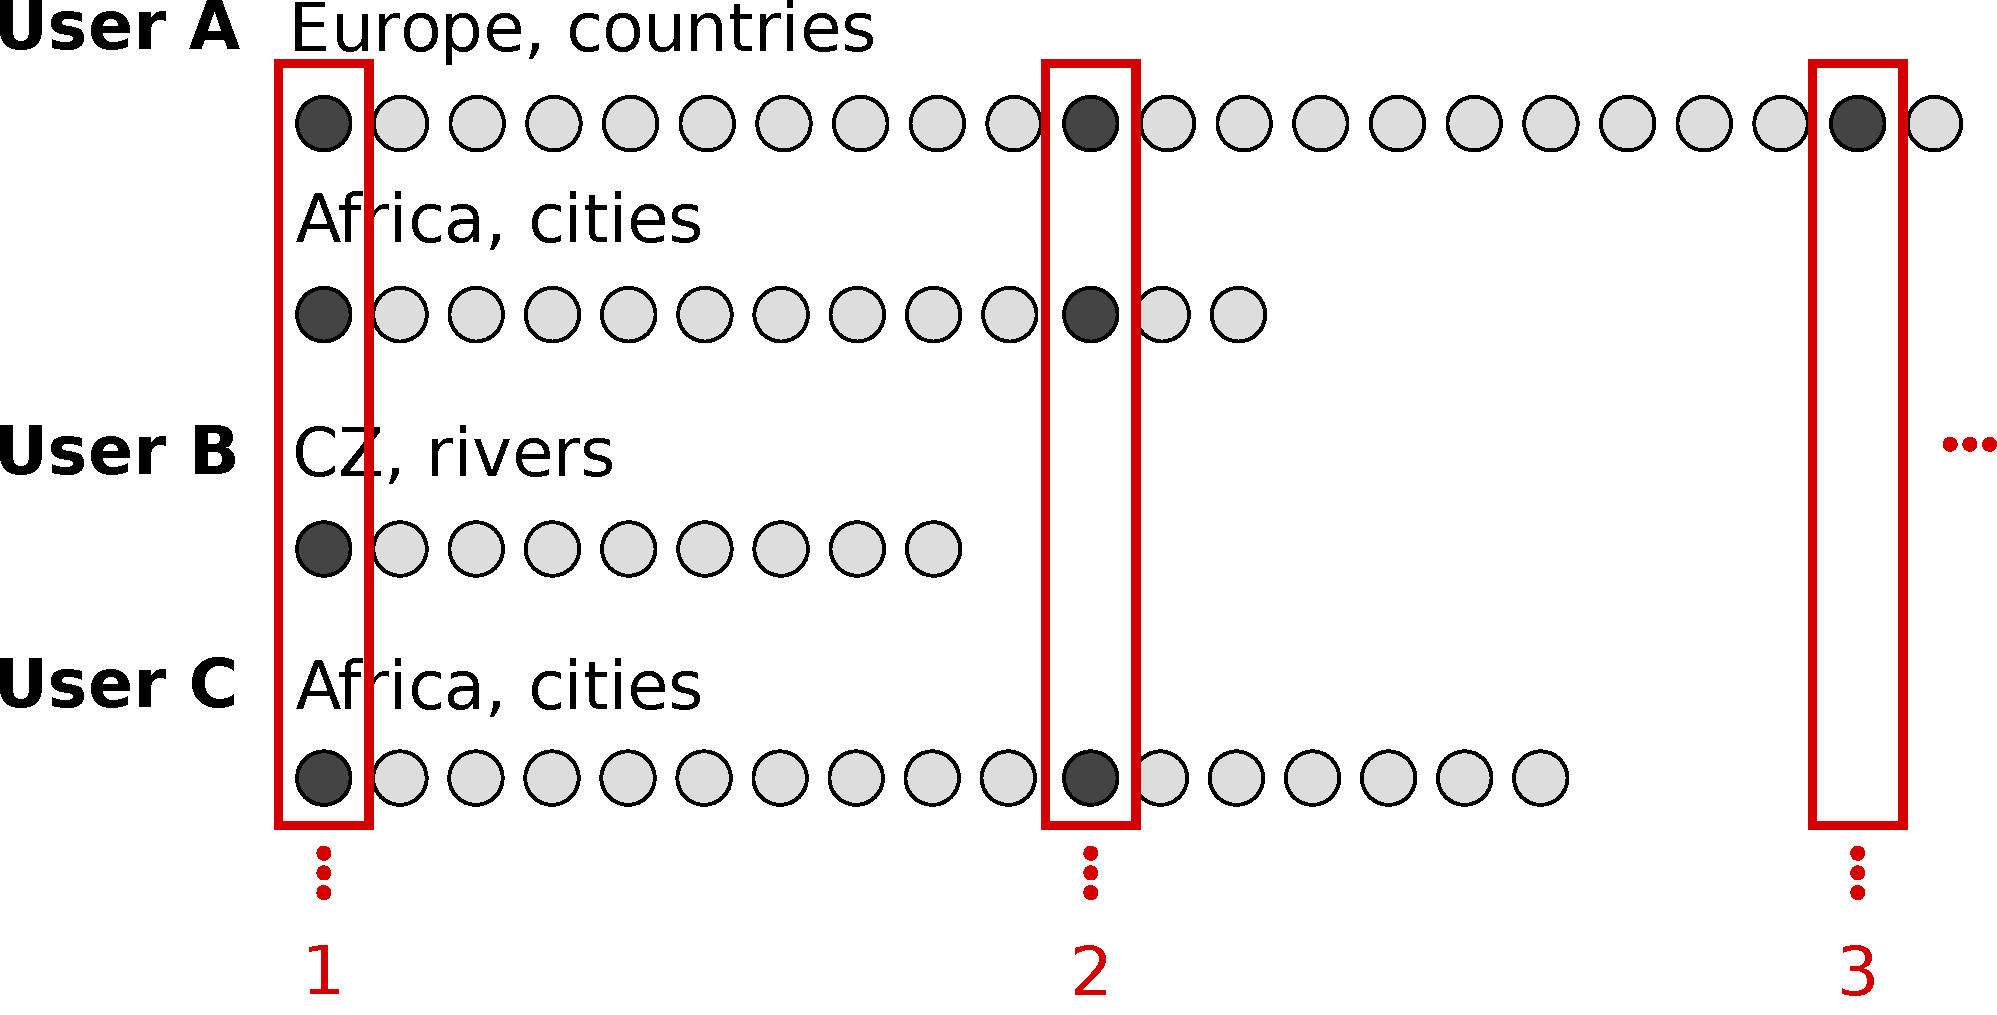
\includegraphics[width=\textwidth]{img/reference_answers_learning}
\end{frame}


\begin{frame}
  \frametitle{Learning curve}
	\begin{itemize}
		\item Power law: $f(x)=ax^{-k}$
		\item $x$ - number of attempts
    \item $a$ - initial error rate
    \item $k$ - learning rate
	\end{itemize}
  \only<1>{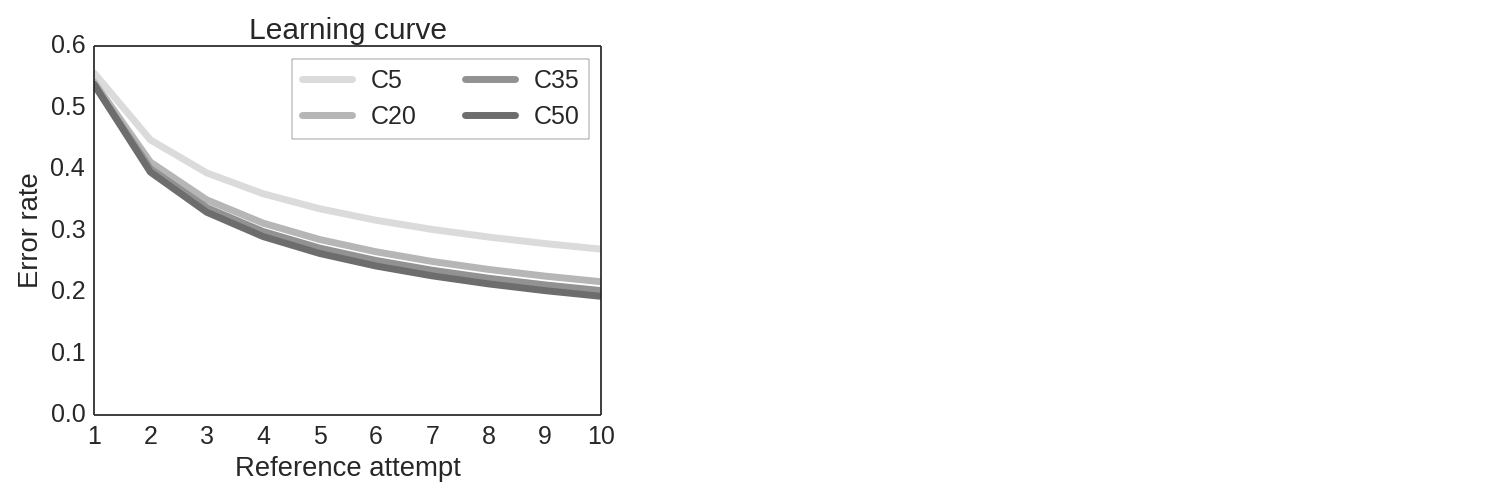
\includegraphics[width=\textwidth]{img/target_difficulty_context_learning_slope_1}}
  \only<2>{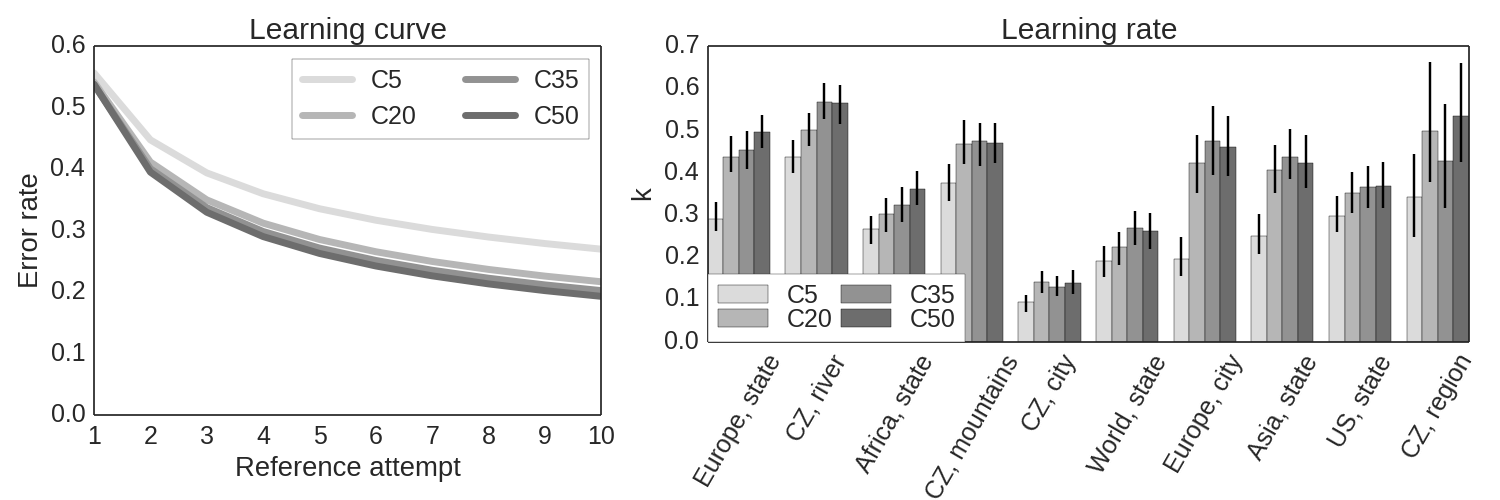
\includegraphics[width=\textwidth]{img/target_difficulty_context_learning_slope}}
\end{frame}

\begin{frame}
  \frametitle{Attrition bias}
  \only<1>{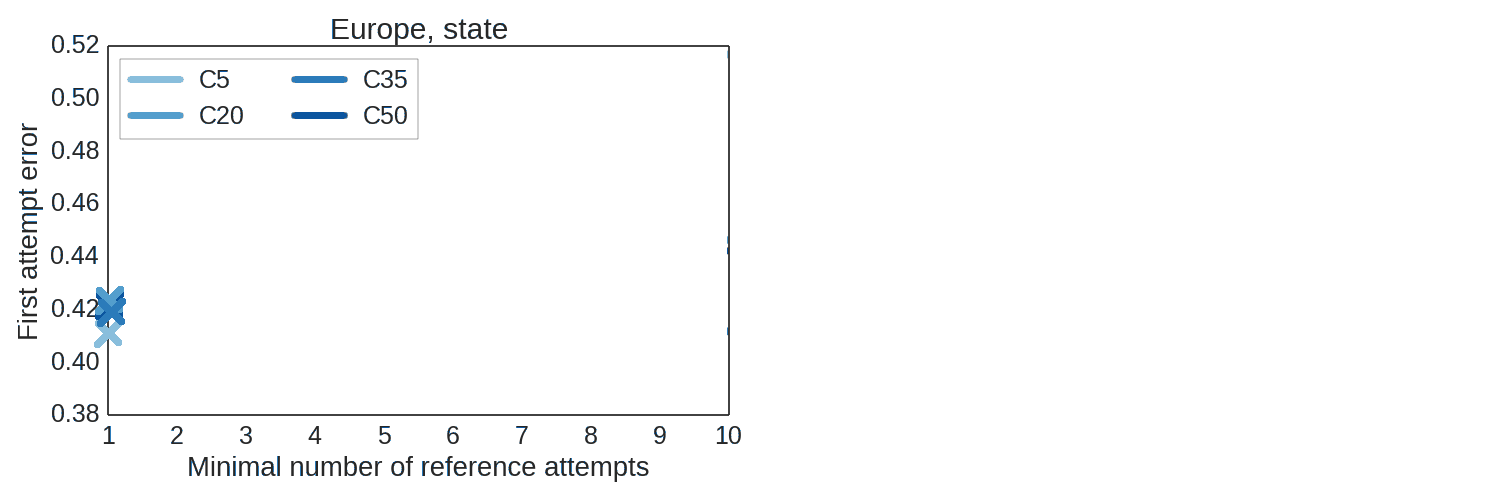
\includegraphics[width=\textwidth]{img/target_difficulty_attrition_bias_contexts_selected_1}}
  \only<2>{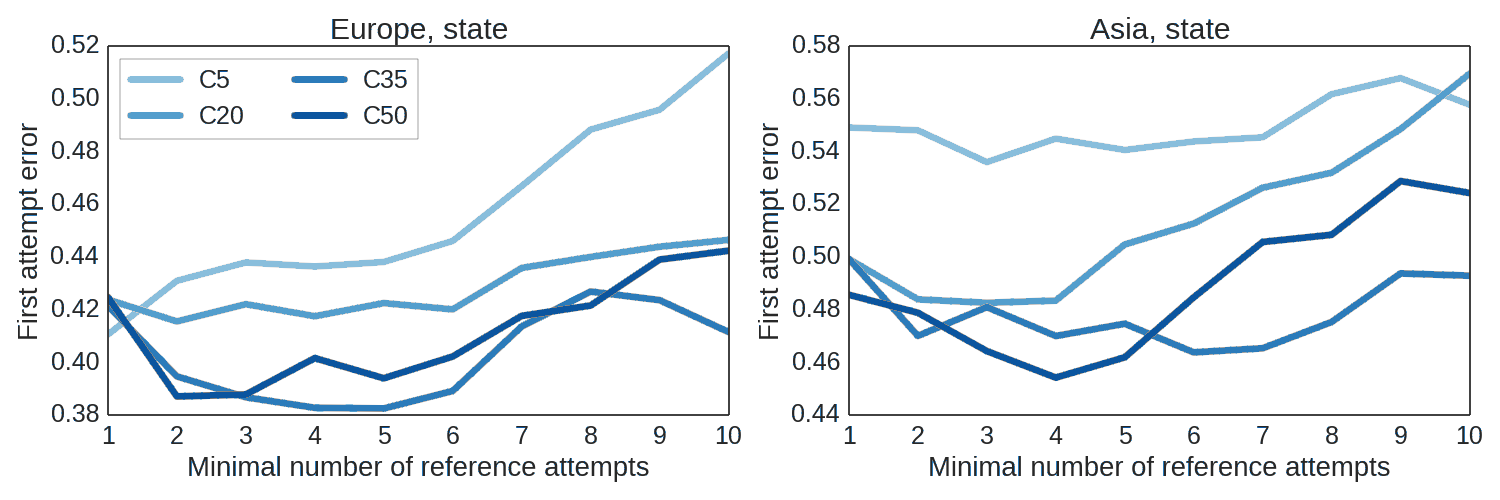
\includegraphics[width=\textwidth]{img/target_difficulty_attrition_bias_contexts_selected}}
\end{frame}

\begin{frame}
  \frametitle{Conclusion}
	\begin{itemize}
		\item Easy questions good for
    \begin{itemize}
      \item Short-term engagement
    \end{itemize}
		\item Difficult questions good for:
    \begin{itemize}
      \item Long-term engagement
      \item Learning 
    \end{itemize}
		\item Methodological issues:
    \begin{itemize}
      \item Short-term vs. long-term engagement
      \item Attrition bias
    \end{itemize}
	\end{itemize}

\end{frame}




\begin{frame}
	\begin{center}
		{\Huge outlinemaps.org}

		\medskip
		(data.outlinemaps.org)

		\bigskip
		\bigskip
		slaweet@mail.muni.cz
	\end{center}
\end{frame}
\end{document}

